
\ifprof
\else

Soit un plan muni d'un repère orthonormé $\left(O,\overrightarrow{i}\overrightarrow{j}\right)$. Soient $n$ points appartenant à ce plan. 
On note $(x_n,y_n)$ les coordonnées du point $P_n$. 

On se donne maintenant un point $A$ de coordonnées $(x_A,y_A)$. Le problème est le suivant : \textbf{déterminer le chemin le plus court démarrant en $A$ et passant une seule fois par chacun des $n$ points $P_n$.}

\begin{multicols}{3}
\begin{center}
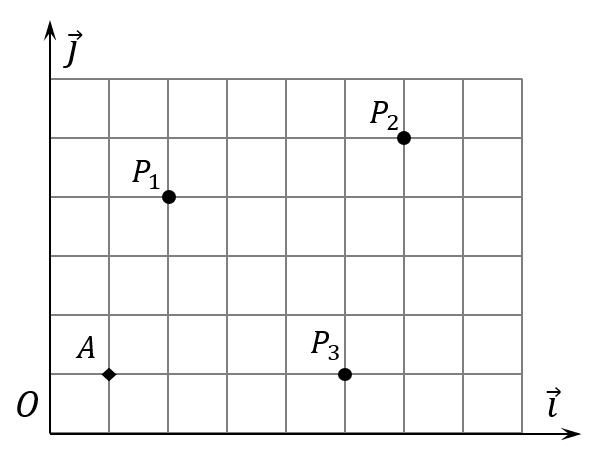
\includegraphics[width=.9\linewidth]{img_01}

Points dans le plan
\end{center}

\begin{center}
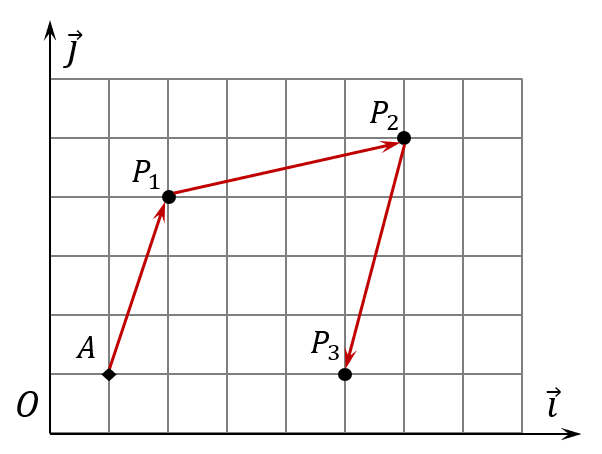
\includegraphics[width=.9\linewidth]{img_02}

Chemin $A\to P_1 \to P_2 \to P_3$
\end{center}

\begin{center}
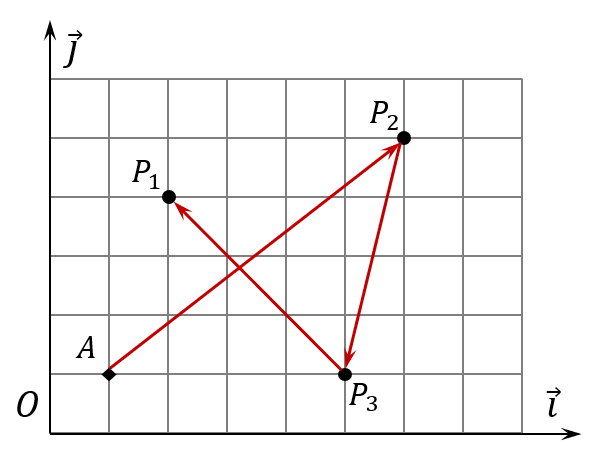
\includegraphics[width=.9\linewidth]{img_03}

Chemin $A\to P_2 \to P_3 \to P_1$
\end{center}
\end{multicols}
\fi

%\subsection*{Réflexions autour de la résolution du problème par force brute}
%
%\question{Dénombrer le nombre de chemins possibles démarrant par $A$ et passant par 3 points.}
%\ifprof
%\begin{corrige}
%6 chemins ($A-P_1-P_2-P_3$, $A-P_1-P_3-P_2$, $A-P_2-P_1-P_3$, $A-P_2-P_3-P_1$, $A-P_3-P_1-P_2$ et $A-P_3-P_2-P_1$).
%\end{corrige}
%\else
%\fi
%
%\question{* Dénombrer le nombre de chemins possibles démarrant par $A$ et passant par 3 points.}
%\ifprof
%\begin{corrige}
%$n!$
%\end{corrige}
%\else
%\fi
%
%\question{Conclure sur le nombre d'opérations (et donc sur le temps de calcul) nécessitant de déterminer la distance de l'ensemble des chemins passant par $n$ points.}
%\ifprof
%\begin{corrige}
%Beaucoup de temps !
%\end{corrige}
%\else
%\fi


\subsection*{Résolution du problème}

\ifprof
\else
Les coordonnées d'un point $P$ sont modélisées en python par une liste de deux coordonnée. Ainisi, un point $P(x_P,y_P)$ sera déclaré par : \texttt{p = [xP,yP]}.

On note \texttt{pts} une liste de $n$ points. On a donc \texttt{pts = [[x1,y1], [x2,y2], ... [xn,yn]]}. 
\fi

\question{Écrire la fonction \texttt{distance(p1:list,p2:list)-> float} permettant de calculer la distance euclidienne entre deux points. Vous importerez les fonctions que vous jugerez utile. La fonction \texttt{Q1\_test()}  permet de valider votre fonction dans un cas.}
\ifprof
\begin{corrige}~\\
\vspace{-.5cm}
\begin{lstlisting}
from math import sqrt
def distance(p1, p2):
    x1, y1 = p1
    x2, y2 = p2
    return sqrt((x1 - x2) ** 2 + (y1 - y2) ** 2)

def distance2(p1, p2): # sans import
    x1, y1 = p1
    x2, y2 = p2
    return ((x1 - x2) ** 2 + (y1 - y2) ** 2)**0.5
\end{lstlisting}
\end{corrige}
\else
\fi
\ifprof
\else
\vspace{.25cm}

On souhaite réaliser un tableau contenant :
\begin{itemize}
\item l'ensemble des distances entre chacun des points \texttt{pts};
\item l'ensemble des distances entre le point $A$ et chacun des points \texttt{pts}.
\end{itemize}

On cherche ainsi à obtenir le tableau des distances suivant. 
\begin{center}
\begin{tabular}{|c|c||c|c|c|c|c|}
\hline 
Points& & $P_1$ & $P_2$ & ... & $P_n$ & $A$ \\ \hline
&index & \texttt{0} & \texttt{1} & ... & \texttt{n-1} & n \\ \hline\hline
$P_1$  & \texttt{0} & \texttt{distance(p1,p1)} & \texttt{distance(p1,p2)} &  ... & \texttt{distance(p1,pn)} & \texttt{distance(p1,a)}  \\ \hline
$P_2$ & \texttt{1} & \texttt{distance(p2,p1)} & \texttt{distance(p2,p2)} &  ... & \texttt{distance(p2,pn)} & \texttt{distance(p2,a)}  \\ \hline
... & ... & ... & ... & ... & ...& ... \\ \hline
$P_n$ & \texttt{n-1} & \texttt{distance(pn,p1)} & \texttt{distance(pn,p2)} &  .. & \texttt{distance(pn,pn)} & \texttt{distance(pn,a)}  \\ \hline
$A$  & \texttt{n} & \texttt{distance(a,p1)} & \texttt{distance(a,p2)} &  .. & \texttt{distance(a,pn)} & \texttt{distance(a,a)}  \\ \hline
\end{tabular}
\end{center}

On aura alors :
\begin{lstlisting}
tab = [[distance(p1,p1), distance (p1,p2), ..., distance(p1,pn),distance(p1,pa)],
          [distance(p2,p1), distance (p2,p2), ..., distance(p2,pn),distance(p2,pa)],
          [... ,... , ..., ..., ...],
          [distance(pn,p1), distance (pn,p2), ..., distance(pn,pn),distance(pn,pa)],
          [distance(pa,p1), distance (pa,p2), ..., distance(pa,pn),distance(pa,pa)]]
\end{lstlisting}
                                        
On note que pour tout point $P$, \texttt{distance(p,p)=0} et que pour tous points $P_1$, $P_2$, \texttt{distance(p1,p2)=distance(p2,p1)}.
\fi

\question{Écrire la fonction \texttt{distances(pts:list,dep:list)-> list} permettant de calculer l'ensemble des distances entre chacun des $n$ points $P$ de la liste \texttt{pts} d'une part. Elle permet d'autre part de calculer  chacune des distances entre le point de départ $A$ (\texttt{dep}) et chacun des points de la listes \texttt{pts} conformément à l'exemple ci-dessus. La fonction \texttt{Q2\_test()} permet de valider votre fonction dans un cas.}
\ifprof
\begin{corrige} ~\\


\begin{lstlisting}
def distances(pts, dep):
    n = len(pts)
    tab = [(n+1)*[0] for i in range(n+1)]
    for i in range(n):
        for j in range(i):
            tab[i][j] = distance(pts[i], pts[j])
            tab[j][i] = tab[i][j]
        tab[n][i] = distance(dep, pts[i])
        tab[i][n] = tab[n][i]
    return tab
\end{lstlisting}
\end{corrige}
\else
\fi


\question{En prenant compte de la note précédente, estimer le nombre de distances à calculer par l'algorithme. }%(Réaliser l'application numérique poiy}
\ifprof
\begin{corrige}
Le tableau des distances contient  $n+1$ lignes et colonnes soit  $(n+1)\times (n+1)$ valeurs. 

Les termes de la diagonale sont tous nuls. Il ne faut donc pas les calculer. Il y en a $n+1$. 

Le tableau est symértrique ce qui signifie que \texttt{tab[i][j]=tab[j][i]}. 

Il faut donc calculer $\dfrac{(n+1)^2-(n+1)}{2}=\dfrac{n(n+1)}{2}$ distances.

\end{corrige}
\else
\fi

\vspace{.25cm}

Soit un chemin, quelconque passant par un ensemble de points contenu dans le tableau des distances. Pour modéliser ce chemin, on utilise la liste des index des points qui le constituent. 
Ainsi si \texttt{chemin = [n,4,0,n-1]} alors c'est qu'on a parcouru le chemin $A\to P_5 \to P_1 \to P_n$. 



\question{Écrire la fonction \texttt{longueur(chemin:list, tab:list) -> float} où \texttt{tab} est un tableau de distances déterminé par la fonction \texttt{distances}. La fonction \texttt{Q4\_test()}  permet de valider votre fonction dans un cas.}
\ifprof
\begin{corrige}~\\ \vspace{-.5cm}
\begin{lstlisting}
def longueur(chemin, dist):
    d = 0
    id_pt = len(dist) - 1
    for point in chemin:
        d = d + dist[id_pt][point]
        id_pt = point
    return d
\end{lstlisting}
\end{corrige}
\else
\fi


\question{Proposer une version récursive de cet algorithme. On la notera \texttt{longueur\_rec(chemin:list, tab:list) -> float}.}
\ifprof
\begin{corrige}~\\  \vspace{-.5cm}
\begin{lstlisting}
def longueur(chemin, dist): A TESTER !!
    d = 0
    if len(chemin) == 2 :
        return distance(chemin[0]chemin[1])
    else : 
        return d + longueur(chemin([1:],dist))
\end{lstlisting}
\end{corrige}
\else
\fi
\ifprof
\else
\vspace{.25cm}


Dans le cadre de l'algorithme glouton, on considère qu'on a atteint le point $k$. On va alors rechercher le point le plus proche parmi les points non visités. On va donc définir la liste des points disponibles. Pour cela, on introduit une liste de booléens \texttt{dispo} de taille $n+1$. Initialement, aucun point n'a été visité, \texttt{dispo} est donc constituée de $n+1$ \texttt{True}. Lorsqu'un point a été visité, l'index du point visité passe à \texttt{False}. 
\fi

\question{On considère que \texttt{dispo=[True, True, False, False, True, False]}. Combien existerait-il de points dans la variable \texttt{pts} définie précédemment ? Combien de points ont été parcouru ? Citer les points visités.}

\ifprof
\begin{corrige}~\\
\texttt{pts} est constitué de 5 points. 
3 points ont été visités : $A$, $P_3$ et $P_4$. 
\end{corrige}
\else
\fi

\ifprof
\else

Pour un point d'indice \texttt{i} on va rechercher l'indice du point le plus proche parmi les points qui n'ont pas été visités.

\begin{center}
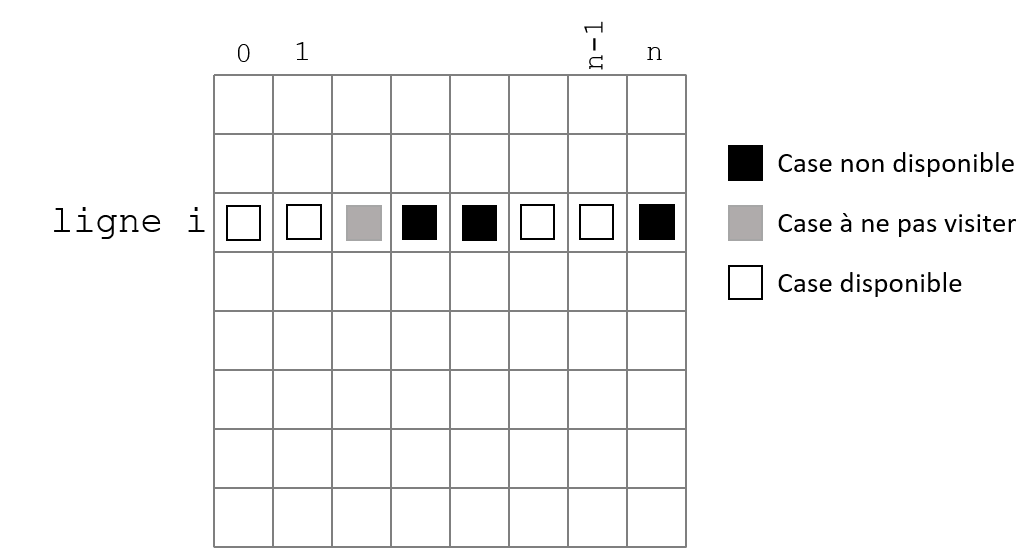
\includegraphics[width=.6\linewidth]{img_04}
\end{center}
\fi


\question{Dans la figure ci-dessus, expliquer pourquoi il y a une case à ne pas visiter ?}
\ifprof
\begin{corrige} 
On ne visite pas la case où on est ...
\end{corrige}
\else
\fi

\question{Écrire une fonction \texttt{indice(i:int, tab:list, dispo:list)->int} permettant de déterminer l'index du point le plus proche du point d'index \texttt{i}, parmi les points disponibles. \texttt{tab} désigne le tableau des distances créé avec la fonction \texttt{distances}. La fonction \texttt{Q8\_test()}  permet de valider votre fonction dans un cas.}
\ifprof
\begin{corrige}~\\ \vspace{-.5cm}
\begin{lstlisting}
def indice(position, dist, dispo):
    n = len(dist) - 1
    global dim
    mini = 3 * dim # supérieur à la diagonale du carré
    for i in range(n):
        if dispo[i]:
            d = dist[position][i]
            if d < mini:
                mini = d
                ind = i
    return ind
\end{lstlisting}
\end{corrige}
\else
\fi

 

\question{Écrire la fonction \texttt{plus\_court\_chemin(dist:list)->list} permettant de construire la chemin le plus court. Le chemin sera constitué de la liste des index des points. On initialisera donc le chemin avec le plus grand index de \texttt{dist}. On initialisera la liste \texttt{dispo} des points disponibles.  \'A chaque itération, on ajoutera à \texttt{chemin} le point le plus proche puis on mettra à jour la variable \texttt{dispo}. }
\ifprof
\begin{corrige}~\\
\vspace{-.5cm}
\begin{lstlisting}
def plus_court_chemin(dist):
    n = len(dist) - 1
    chemin = []
    dispo = n * [True]
    position = n
    while len(chemin) < n:
        position = indice(position, dist, dispo)
        chemin.append(position)
        dispo[position] = False
    return chemin
\end{lstlisting}
\end{corrige}
\else
\fi


\subsection*{Représentation du chemin}

\question{Tester le fonction \texttt{plot\_chemin()}. Commenter l'ensemble des lignes en effectuant les regroupements vous paraissant nécessaires.}
%
% \lstset{numbers=left,
%    stepnumber=1}
%
%\begin{lstlisting}
%import matplotlib.pyplot as plt
%
%x = [u[0] for u in pts]
%y = [u[1] for u in pts]
%plt.plot(x, y, "x")
%plt.plot(depart[0], depart[1], "+")
%plt.show()
%
%tableau = distances(pts, depart)
%ch = plus_court(tableau)
%print(longueur(ch, tableau))
%
%xliste = [depart[0]] + [pts[k][0] for k in ch]
%yliste = [depart[1]] + [pts[k][1] for k in ch]
%plt.plot(x, y, "x") # affichage des points
%plt.plot(depart[0], depart[1], "+")
%plt.plot(xliste, yliste) # affichage du chemin
%plt.show()
%\end{lstlisting}
